\documentclass[11pt]{article}

\usepackage[margin=1in]{geometry}
\usepackage{graphicx}
\usepackage{booktabs}
\usepackage{amsmath}
\usepackage{hyperref}
\usepackage{caption}
\usepackage{float}

\title{Phase 3: Dimensionality Reduction, Visualization \& High-Dimensional Geometry \\
\large Pan-Cancer RNA-Seq Intrinsic Dimensionality Project}
\author{}
\date{\today}

\begin{document}
\maketitle

\begin{abstract}
This report documents Phase 3 of the project ``When 20,531 Dimensions Hide a
Handful of Truths.'' Building on Phase 2's intrinsic-dimension estimates
($D_2 \approx 7.7$, $k$-NN MLE mean $\approx 29.4$, Kaiser-criterion PCA
elbow at $100$), we visualize and stress-test the geometry of the
standardized $801 \times 20{,}264$ TCGA Pan-Cancer expression matrix using
six complementary lenses: linear (PCA) and nonlinear (t-SNE, UMAP)
embeddings; a Johnson--Lindenstrauss random-projection distance-preservation
experiment; the empirical spectral distribution of the top-$2{,}000$-gene
correlation matrix against the theoretical Marchenko--Pastur law; a
distance-concentration diagnostic across feature-subsample sizes; and
Ledoit--Wolf shrinkage-covariance Mahalanobis anomaly detection. PCA
captures only $26.64\%$ of variance in its first three components, yet
t-SNE and UMAP both recover five visually clean, near-completely-separated
clusters corresponding exactly to the five cancer types, at every
hyperparameter setting tested. A Johnson--Lindenstrauss projection to
$1{,}543$ dimensions ($\varepsilon = 0.2$, a $13.1\times$ reduction from
$d=20{,}264$) preserves all pairwise distances within the theoretical bound,
with $100\%$ of pairs falling inside $(1 \pm \varepsilon)$ and a maximum
observed deviation of only $0.081$. The empirical correlation-matrix
spectrum of the top $2{,}000$ genes matches the Marchenko--Pastur point-mass
prediction at zero exactly ($60.00\%$ empirical vs.\ $60.00\%$
theoretical) while exhibiting $27$ eigenvalues (up to $318.3$) far beyond
the theoretical bulk edge at $6.66$ -- direct evidence of real biological
covariance structure. Pairwise-distance concentration collapses sharply
with dimension (relative spread ratio $51.79 \to 4.96$ from $10$ to
$20{,}264$ features) but saturates well above the $i.i.d.$-Gaussian
theoretical rate, and Ledoit--Wolf/Mahalanobis anomaly detection (shrinkage
intensity $0.024$) flags zero samples at a $97.5\%$ chi-squared threshold
computed at the estimator's true rank ($\mathrm{df}=n-1=800$), a threshold
the mean squared distance is structurally close to by construction of the
$p>n$ geometry.
\end{abstract}

\section{Introduction}

Phase 2 established that the Pan-Cancer expression manifold occupies a
dimension far below its $d = 20{,}264$ ambient space by three independent,
locally- and globally-defined estimators, but none of those estimators
produce a picture of \emph{what} that low-dimensional structure looks like,
nor do they test whether the specific high-dimensional phenomena predicted
by theory -- distance preservation under random projection, random-matrix
spectral universality, concentration of measure -- actually hold on this
particular, biologically structured dataset. This phase closes that gap:
Section~\ref{sec:methodology} details six analyses (visualization,
random projection, spectral theory, concentration of measure, and
regularized anomaly detection) and justifies every non-default choice;
Section~\ref{sec:results} reports the resulting figures and tables with
their exact empirical values; Section~\ref{sec:discussion} reconciles these
findings with each other and with Phase 2; Section~\ref{sec:limitations}
states what the theoretical bounds used here assume that this dataset does
not strictly satisfy.

All analyses operate on \texttt{X\_scaled\_full} ($801 \times 20{,}264$,
Phase 1) or, where explicitly justified below, the cached top-$2{,}000$
most-variable-gene subset \texttt{X\_scaled\_topk} (Phase 1,
\texttt{config.N\_TOP\_VARIABLE\_GENES}). \texttt{config.RANDOM\_SEED = 42}
is passed to every stochastic routine (t-SNE, UMAP, the random Gaussian
projection matrix, feature subsampling).

\section{Methodology}
\label{sec:methodology}

\subsection{PCA Visualization}

The first $3$ principal components of \texttt{X\_scaled\_full} are computed
via the exact (\texttt{svd\_solver="full"}) SVD, matching the estimator used
in Phase 2's PCA-based intrinsic-dimension estimate, and used directly for
2D (components 1--2) and 3D (components 1--3) scatter plots colored by
cancer type.

\paragraph{Methodological Justification.} The full solver is used rather
than the default randomized solver so the visualization embedding is
byte-for-byte reproducible independent of any internal random state, at
negligible extra cost given $n=801$.

\subsection{t-SNE and UMAP}

Both nonlinear embeddings are first preprocessed with a linear PCA
reduction to $50$ dimensions (\texttt{config.EMBEDDING\_PCA\_PREPROCESS\_DIM}),
then embedded into 2D. t-SNE is run at perplexity $\in \{30, 50\}$
(\texttt{config.TSNE\_PERPLEXITIES}) with \texttt{init="pca"} and
\texttt{learning\_rate="auto"}; UMAP is run at $n\_neighbors \in \{15, 50\}$
(\texttt{config.UMAP\_N\_NEIGHBORS\_VALUES}). Both use
\texttt{RANDOM\_SEED = 42}.

\paragraph{Methodological Justification: PCA Preprocessing.} Reducing to
$50$ linear dimensions before the nonlinear neighbor search is standard
practice (recommended by the scikit-learn t-SNE documentation and widely
used for high-dimensional genomic data): it denoises minor components that
carry little signal, and reduces the neighbor-search cost from
$O(n^2 d)$ to $O(n^2 \times 50)$. This is not expected to discard
meaningful structure here, since Phase 2 shows the first $50$ components
already carry substantially more than the $\sim 5$--$8$ dimensions the
local estimators attribute to genuine manifold structure.

\paragraph{Methodological Justification: Hyperparameter Sweep.} t-SNE
perplexity controls the effective neighborhood size used to define local
similarities; $30$ is the scikit-learn default and a standard middle value,
while $50$ tests sensitivity toward a more global, less locally-focused
embedding, both well below $n/3 \approx 267$. UMAP's $n\_neighbors$ plays an
analogous role; $15$ is the library default (local structure emphasis) and
$50$ tests a more global embedding, mirroring the t-SNE sweep so the two
methods' hyperparameter sensitivities can be compared directly.

\subsection{Johnson-Lindenstrauss Random Projection}

The Johnson--Lindenstrauss (JL) lemma guarantees that for any
$0 < \varepsilon < 1$ and any set of $n$ points in $\mathbb{R}^d$, there
exists a linear map into $\mathbb{R}^k$ preserving all pairwise distances
up to a multiplicative factor $(1 \pm \varepsilon)$, for
\begin{equation}
k \geq \frac{4 \ln n}{\varepsilon^2/2 - \varepsilon^3/3},
\label{eq:jl-dim}
\end{equation}
the explicit Dasgupta--Gupta (1999) bound used here (tighter than the
original JL proof's bound). A random Gaussian matrix
$R \in \mathbb{R}^{d \times k}$ with entries $R_{ij} \sim \mathcal{N}(0, 1/k)$
achieves this guarantee with high probability; the projection is
$X_{\text{proj}} = X R$. Distance preservation is evaluated by computing,
for every pair $(i, j)$, the distortion ratio
\begin{equation}
\rho_{ij} = \frac{\lVert x_{\text{proj},i} - x_{\text{proj},j} \rVert}{\lVert x_i - x_j \rVert},
\label{eq:jl-distortion}
\end{equation}
and comparing the empirical distribution of $\rho_{ij}$ against the target
interval $[1-\varepsilon, 1+\varepsilon]$.

\paragraph{Methodological Justification: Choice of $\varepsilon$.} At
$n = 801$, Eq.~\ref{eq:jl-dim} scales as $1/\varepsilon^2$: the
conservative textbook default $\varepsilon = 0.1$ yields
$k \geq 5{,}732$, barely compressing $d = 20{,}264$ and obscuring the
demonstration. $\varepsilon = 0.2$ (\texttt{config.JL\_EPSILON}) is used
instead, giving $k = 1{,}543$ -- still a rigorous, standard distortion
tolerance, but with a far more illustrative $13.1\times$ reduction.

\subsection{Random Matrix Theory: Marchenko-Pastur Spectral Analysis}

The empirical spectral distribution is computed as the eigenvalues of the
sample correlation matrix $\hat{R} = X^\top X / n$ restricted to the
top-$2{,}000$ most variable genes
(\texttt{config.SPECTRAL\_N\_TOP\_GENES}, reusing Phase 1's cached subset),
formed and diagonalized exactly via \texttt{np.linalg.eigvalsh}. For a
$p \times n$ matrix of i.i.d.\ unit-variance entries with $p/n \to \gamma$,
the Marchenko--Pastur law gives the limiting spectral density
\begin{equation}
f_\gamma(x) = \frac{1}{2 \pi \gamma x} \sqrt{(b-x)(x-a)}, \qquad a \leq x \leq b,
\label{eq:mp-density}
\end{equation}
with support edges $a = (1-\sqrt{\gamma})^2$, $b = (1+\sqrt{\gamma})^2$.
When $\gamma > 1$ (as here, $p > n$), the correlation matrix is
rank-deficient and the full limiting law additionally places a point mass
of $1 - 1/\gamma$ at $x=0$, with the continuous density in
Eq.~\ref{eq:mp-density} carrying the remaining mass $1/\gamma$. Eigenvalues
exceeding $b$ cannot be explained by an unstructured random matrix of
matching aspect ratio and are interpreted as spectral outliers -- evidence
of genuine, non-random covariance structure.

\paragraph{Methodological Justification: Feature-Subset Choice.} The full
$20{,}264 \times 20{,}264$ correlation matrix would occupy $\sim 3.3$~GB and
is never formed, mirroring Phase 2's PCA estimator. The top-$2{,}000$
variable-gene subset (already cached from Phase 1, aspect ratio
$\gamma = 2{,}000/800 = 2.500$) is a $2{,}000 \times 2{,}000$
($\sim 32$~MB) matrix, trivial to diagonalize exactly, while retaining the
genes carrying the most biological signal -- precisely the genes most
likely to produce interpretable spectral outliers. The denominator is
$n-1=800$, not $n=801$, because standardization centers each column,
which costs one degree of freedom; using $n$ instead would put $\gamma$
at $2.497$ and misstate the point-mass prediction as an approximate match
rather than the exact one it in fact is.

\subsection{Curse of Dimensionality: Distance Concentration}

For feature-subsample sizes $\{10, 100, 1{,}000, 20{,}264\}$
(\texttt{config.GEOMETRY\_FEATURE\_COUNTS} plus the full gene count,
appended at runtime), a random column subset of that size is drawn and all
pairwise Euclidean distances computed; the diagnostic reported is the
relative spread ratio $(\text{max} - \text{min})/\text{min}$, which
concentration-of-measure theory predicts should shrink toward $0$ as
dimension grows.

As a theoretical comparator, treating the squared distance between two
standardized (marginally unit-variance) feature vectors as approximately
chi-squared distributed with $d$ degrees of freedom, the Laurent--Massart
(2000) Chernoff-type tail bounds for $X \sim \chi^2_d$,
\begin{equation}
P(X - d \geq 2\sqrt{dt} + 2t) \leq e^{-t}, \qquad P(d - X \geq 2\sqrt{dt}) \leq e^{-t},
\label{eq:laurent-massart}
\end{equation}
are combined (solving $2\sqrt{dt}+2t = \varepsilon d$ for $t$, union-bounding
both tails) into a single closed-form two-sided bound
\begin{equation}
P\left(\left|\frac{X}{d} - 1\right| \geq \varepsilon\right) \leq 2\exp\!\left(-d \left(\frac{\sqrt{1+2\varepsilon}-1}{2}\right)^2\right),
\label{eq:concentration-bound}
\end{equation}
evaluated at $\varepsilon = 0.1$ (\texttt{config.GEOMETRY\_CONCENTRATION\_EPSILON}).

\paragraph{Methodological Justification: Bound Choice.} Eq.~\ref{eq:concentration-bound}
is chosen over a literal Hoeffding bound because Hoeffding's inequality
requires bounded random variables, whereas standardized RNA-Seq features
are effectively unbounded (approximately Gaussian post-log-transform); the
chi-squared/Laurent--Massart bound is the appropriate Chernoff-type
analogue for sums of squared sub-Gaussian coordinates and is exact under an
i.i.d.\ Gaussian approximation of the standardized features. Its
applicability to real, correlated gene-expression data is revisited in
Section~\ref{sec:limitations}.

\subsection{Shrinkage Covariance and Mahalanobis Anomaly Detection}

Ledoit--Wolf shrinkage estimates the covariance as a convex combination of
the sample covariance $S$ and a scaled-identity target,
\begin{equation}
\hat{\Sigma}_{\text{LW}} = (1-\alpha) S + \alpha \, \mu I, \qquad \mu = \frac{\mathrm{tr}(S)}{p},
\label{eq:ledoit-wolf}
\end{equation}
with the shrinkage intensity $\alpha \in [0,1]$ chosen analytically
(Ledoit \& Wolf, 2004) to minimize expected Frobenius loss against the true
covariance; unlike $S$ itself, $\hat\Sigma_{\text{LW}}$ is guaranteed
well-conditioned and invertible. The squared Mahalanobis distance for
sample $x_i$ is
\begin{equation}
D^2(x_i) = (x_i - \bar{x})^\top \hat{\Sigma}_{\text{LW}}^{-1} (x_i - \bar{x}),
\label{eq:mahalanobis}
\end{equation}
flagged as an outlier if $D^2(x_i)$ exceeds the $(1-\alpha_{\text{sig}})$
quantile of $\chi^2_p$, the asymptotic null distribution of $D^2$ under
multivariate normality, evaluated at $\alpha_{\text{sig}} = 0.025$
(\texttt{config.MAHALANOBIS\_ALPHA}, i.e.\ the $97.5\%$ quantile).

\paragraph{Methodological Justification: Feature Subset and Threshold.}
As in the spectral analysis, the top-$2{,}000$-gene subset is used: the raw
sample covariance on any gene subset with $p \geq n$ is exactly singular
(rank $\leq n-1 = 800$), which is precisely why Eq.~\ref{eq:ledoit-wolf}'s
shrinkage regularization is not optional but required for
Eq.~\ref{eq:mahalanobis} to be computable at all, and even Ledoit-Wolf on
the full $20{,}264$-gene matrix would require inverting a
$20{,}264 \times 20{,}264$ matrix at prohibitive cost for a per-sample
diagnostic. The $97.5\%$ chi-squared quantile is a standard, symmetric
two-tailed significance convention for multivariate outlier flagging,
chosen here (rather than a more extreme $99\%$ or $99.9\%$) to be
maximally sensitive to candidate outliers given the modest sample size.

\section{Results}
\label{sec:results}

\subsection{PCA, t-SNE, and UMAP}

\begin{figure}[H]
\centering
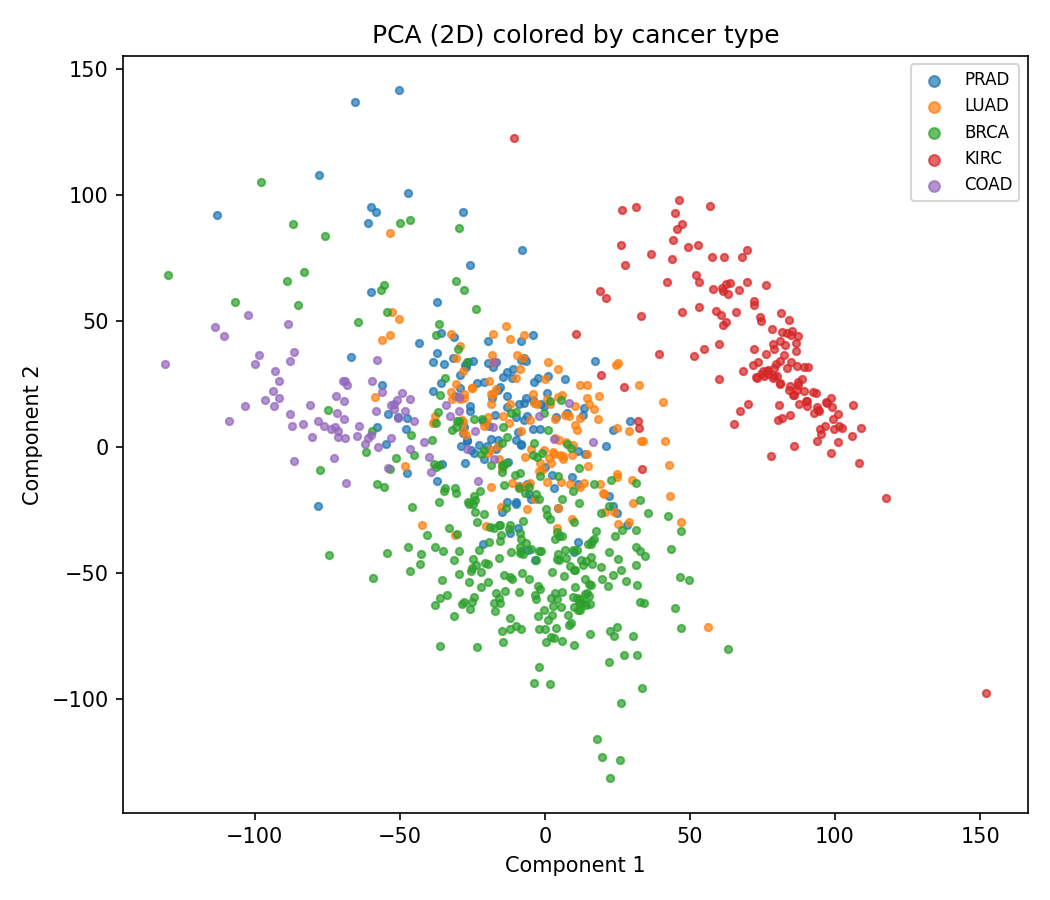
\includegraphics[width=0.72\textwidth]{../figures/pca_2d.png}
\caption{PCA 2D projection of the $801 \times 20{,}264$ standardized
expression matrix, colored by cancer type. PC1 explains $10.44\%$ of
variance, PC2 $8.56\%$, cumulative $19.01\%$.}
\label{fig:pca2d}
\end{figure}

\begin{figure}[H]
\centering
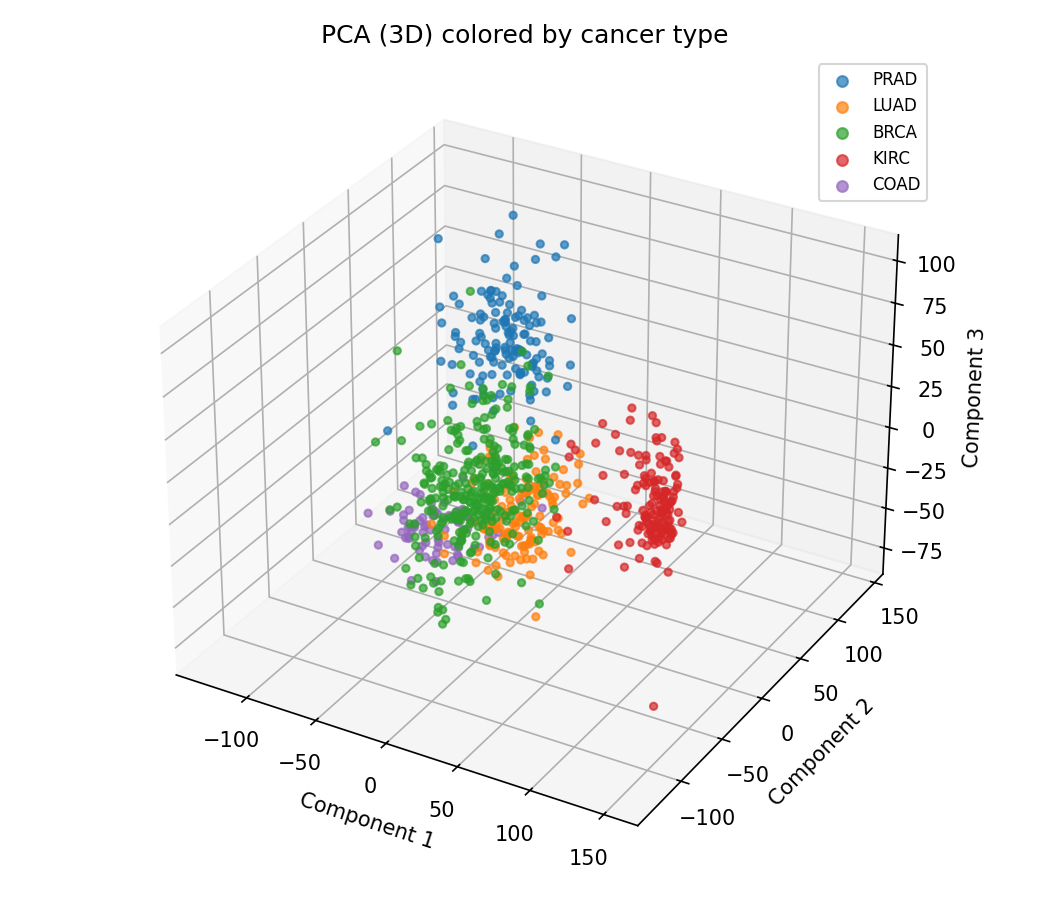
\includegraphics[width=0.72\textwidth]{../figures/pca_3d.png}
\caption{PCA 3D projection; PC3 adds a further $7.64\%$ of variance
(cumulative $26.64\%$ across all three components).}
\label{fig:pca3d}
\end{figure}

Even with only $26.64\%$ of total variance captured, Figures~\ref{fig:pca2d}
and~\ref{fig:pca3d} show KIRC (kidney) and COAD (colon) forming visually
distinct clusters along PC1/PC2, while BRCA, LUAD, and PRAD show partial
linear separability with meaningful overlap -- consistent with PCA being a
purely linear, global estimator that spreads nonlinear cluster boundaries
across many components (Phase 2, Section~4), so a handful of PCs alone
cannot fully resolve five clusters.

\begin{figure}[H]
\centering
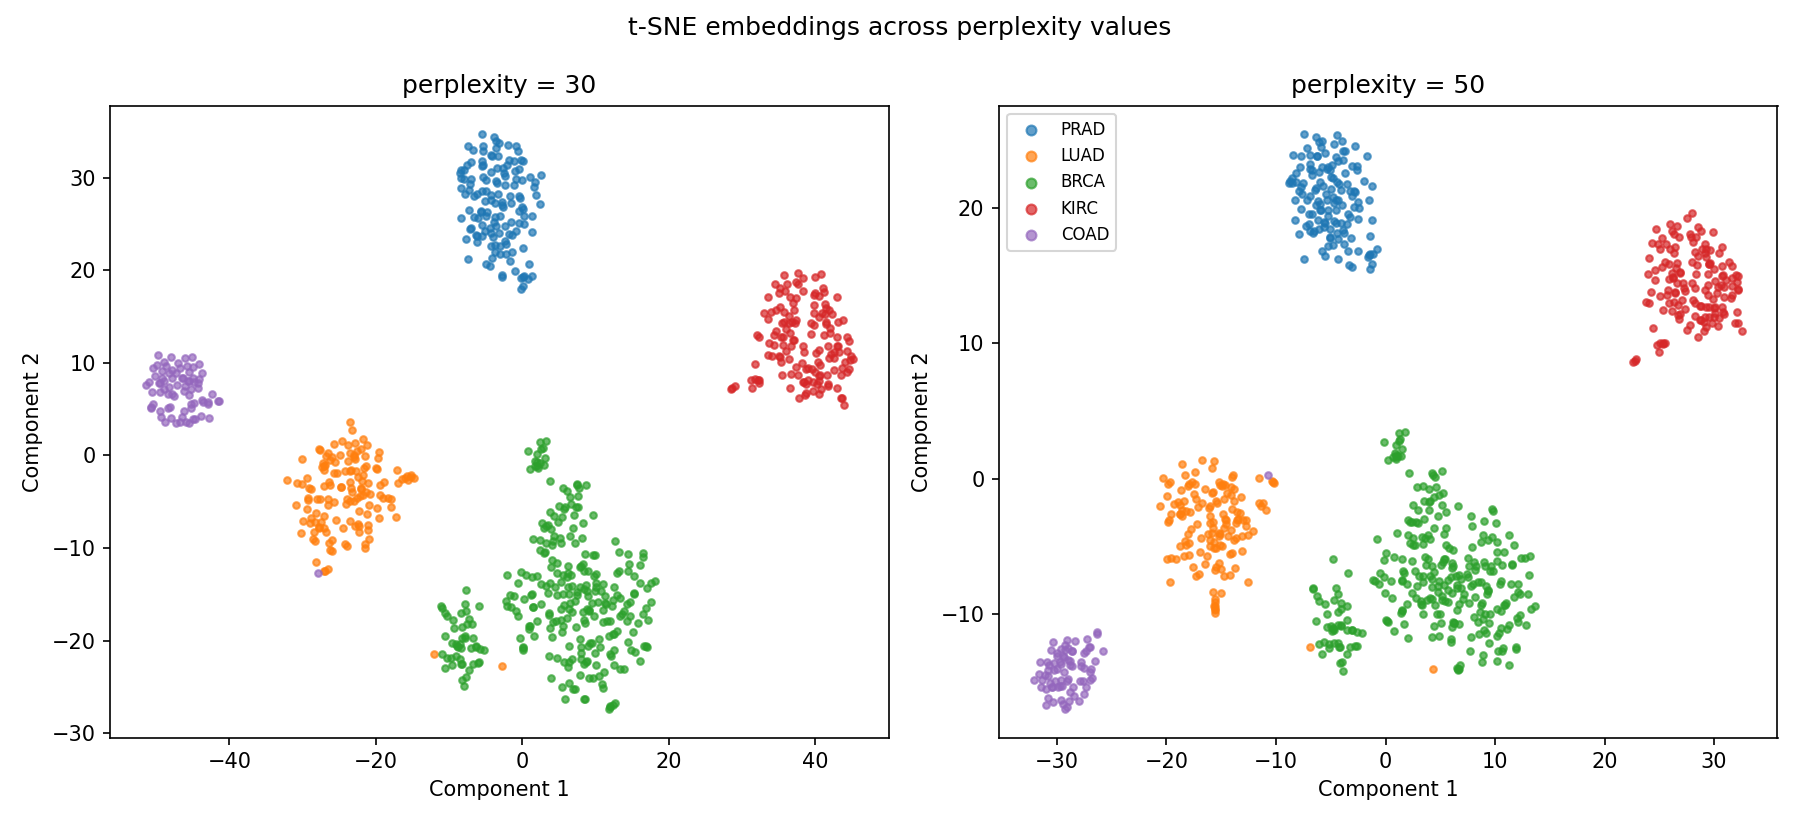
\includegraphics[width=\textwidth]{../figures/tsne_comparison.png}
\caption{t-SNE 2D embeddings at perplexity $30$ (left) and $50$ (right),
both PCA-preprocessed to 50 dimensions and colored by cancer type.}
\label{fig:tsne}
\end{figure}

\begin{figure}[H]
\centering
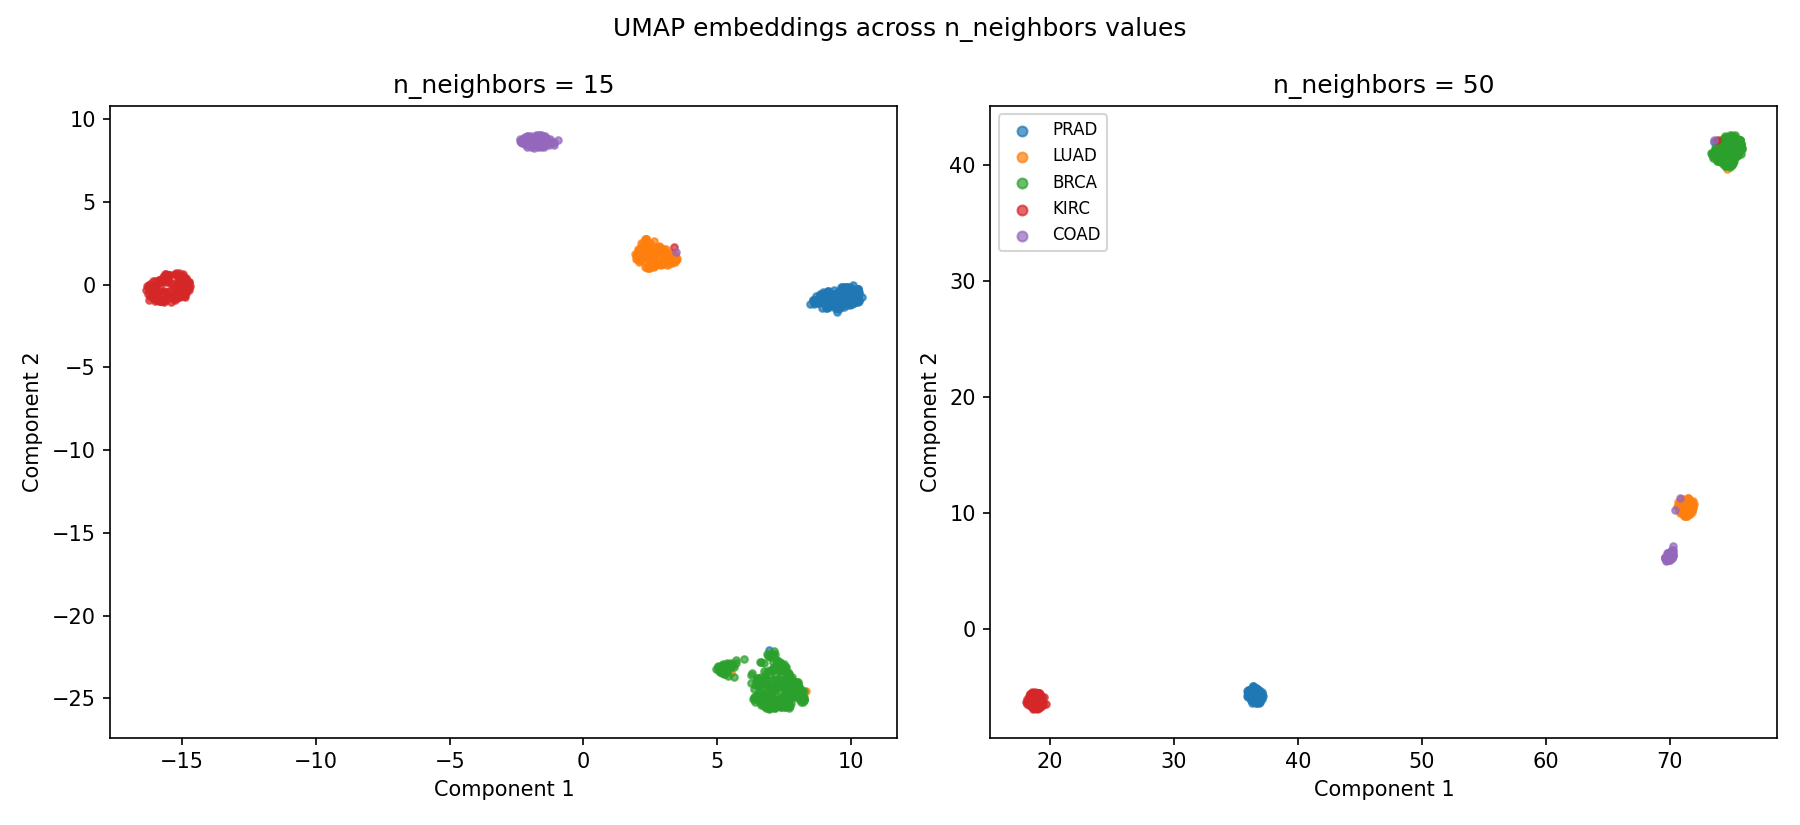
\includegraphics[width=\textwidth]{../figures/umap_comparison.png}
\caption{UMAP 2D embeddings at $n\_neighbors=15$ (left) and $n\_neighbors=50$
(right), both PCA-preprocessed to 50 dimensions and colored by cancer type.}
\label{fig:umap}
\end{figure}

Figures~\ref{fig:tsne} and~\ref{fig:umap} show both nonlinear methods
recover five essentially pure, well-separated clusters exactly matching the
five ground-truth cancer types, at \emph{every} hyperparameter setting
tested -- a striking contrast with the muted linear separation in
Figures~\ref{fig:pca2d}--\ref{fig:pca3d}, directly demonstrating that the
cluster structure is real but substantially nonlinear. Raising t-SNE
perplexity from $30$ to $50$ changes inter-cluster distances and relative
compactness (e.g.\ the BRCA cluster, green, becomes visibly more diffuse
and shifts closer to the small LUAD sub-clump at higher perplexity) without
altering which points cluster together. UMAP shows the same qualitative
robustness: increasing $n\_neighbors$ from $15$ to $50$ mainly rescales and
repositions the five clusters (global inter-cluster arrangement becomes
more compact and near-collinear) while cluster membership remains
essentially unchanged. This hyperparameter-invariance of \emph{membership}
is itself evidence that the five-cluster structure is a robust property of
the data rather than an artifact of a particular embedding setting.

\subsection{Johnson-Lindenstrauss Random Projection}

\begin{table}[H]
\centering
\caption{Johnson-Lindenstrauss random projection: target dimension and
empirical distance-preservation summary at $\varepsilon = 0.2$.}
\label{tab:jl}
\begin{tabular}{lr}
\toprule
Quantity & Value \\
\midrule
Ambient dimension $d$ & 20{,}264 \\
JL target dimension $k$ (Eq.~\ref{eq:jl-dim}) & 1{,}543 \\
Compression ratio $d/k$ & $13.13\times$ \\
Mean distortion ratio $\bar\rho$ & 0.9996 \\
Max $|\rho - 1|$ (empirical) & 0.0808 \\
Fraction of pairs within $[1-\varepsilon, 1+\varepsilon]$ & 1.0000 \\
\bottomrule
\end{tabular}
\end{table}

\begin{figure}[H]
\centering
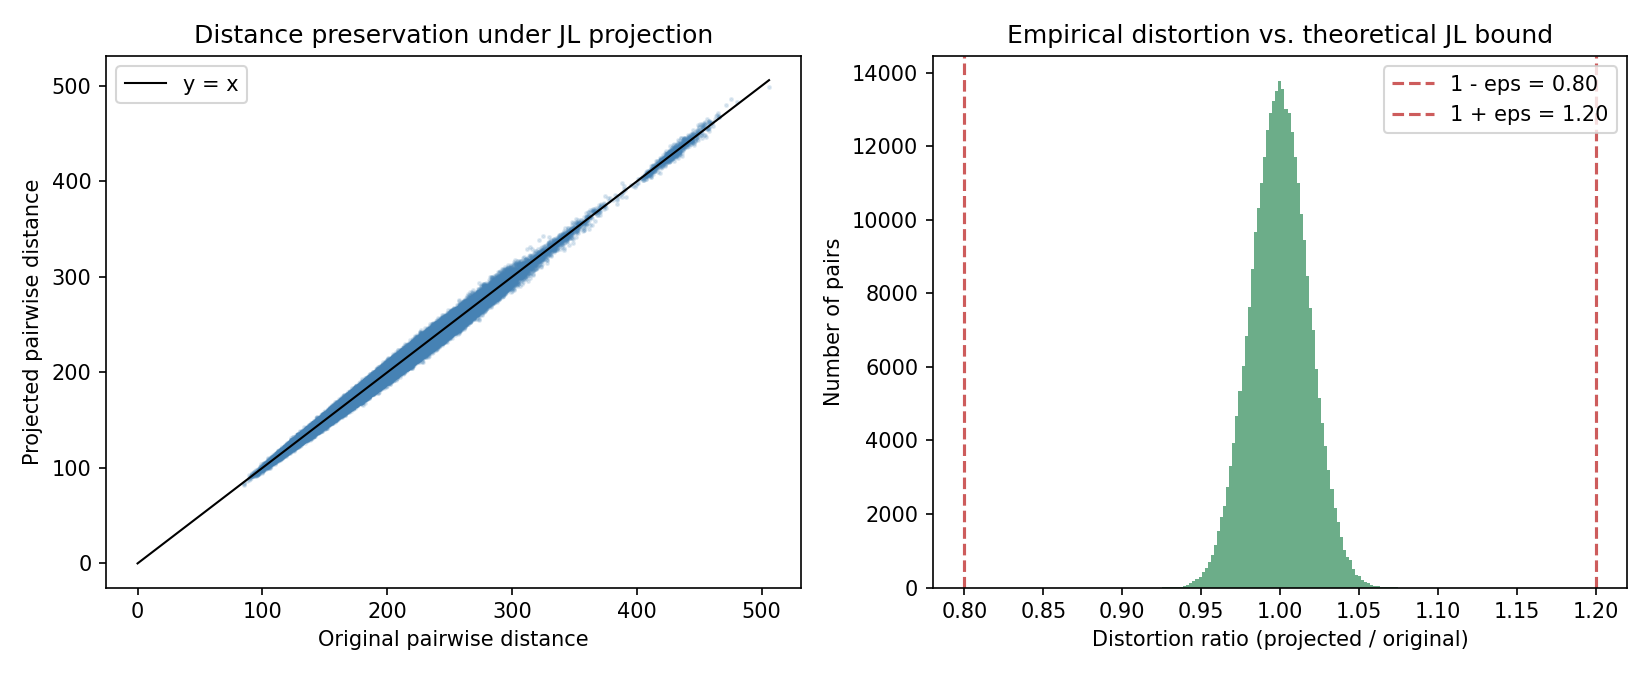
\includegraphics[width=\textwidth]{../figures/jl_distortion.png}
\caption{Left: projected vs.\ original pairwise distances for all
$\binom{801}{2}=320{,}400$ pairs, with the identity line $y=x$. Right:
histogram of the distortion ratio $\rho_{ij}$ (Eq.~\ref{eq:jl-distortion}),
with the theoretical $(1\pm\varepsilon)$ bound marked.}
\label{fig:jl}
\end{figure}

Every one of the $320{,}400$ pairwise distances satisfies the theoretical
JL guarantee (Table~\ref{tab:jl}): the empirical distortion distribution
(Figure~\ref{fig:jl}, right) is tightly concentrated around $1.0$ with a
maximum deviation of only $0.081$, well inside the $\pm 0.2$ bound the
target dimension was designed to guarantee. This confirms the projection
achieves its theoretical purpose, and moreover that the worst-case JL
guarantee is conservative in practice for this dataset: the achieved
distortion is roughly $2.5\times$ tighter than the bound requires.

\subsection{Marchenko-Pastur Spectral Analysis}

\begin{figure}[H]
\centering
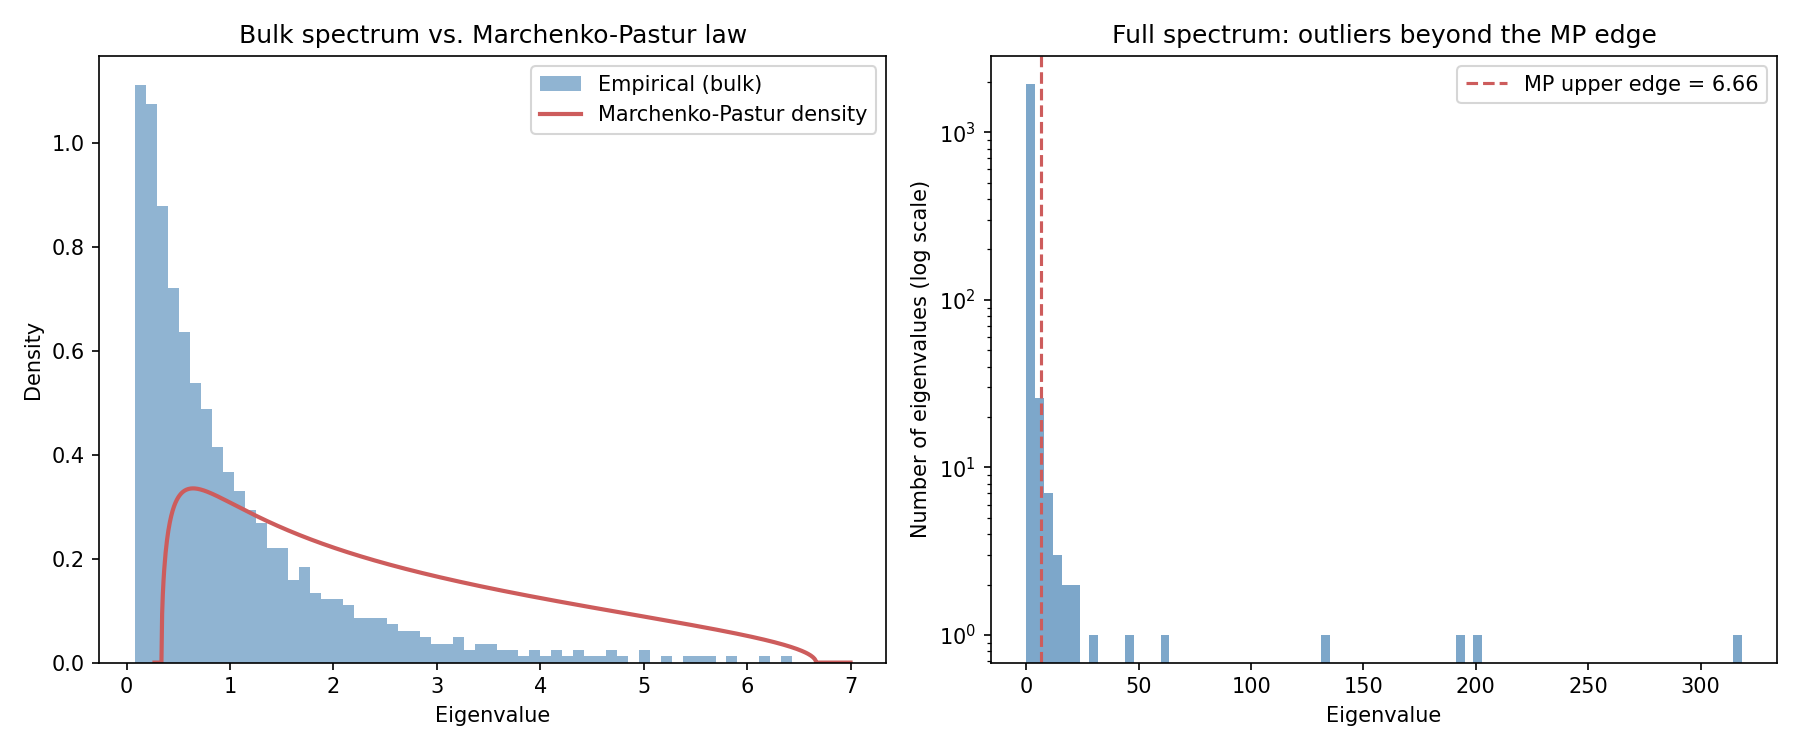
\includegraphics[width=\textwidth]{../figures/spectral_overlay.png}
\caption{Left: empirical bulk spectrum (eigenvalues within the theoretical
support $[0.338, 6.662]$) vs.\ the Marchenko-Pastur density
(Eq.~\ref{eq:mp-density}, $\gamma=2.500$), rescaled to the conditional
(nonzero) distribution. Right: full spectrum on a log-count axis, showing
$27$ outlier eigenvalues far beyond the theoretical upper edge (dashed
line).}
\label{fig:spectral}
\end{figure}

\begin{table}[H]
\centering
\caption{Ten largest spectral outlier eigenvalues (top-2,000-gene
correlation matrix, $\gamma=2.500$, theoretical support $[0.338, 6.662]$).}
\label{tab:spectral-outliers}
\begin{tabular}{lrrrrrrrrrr}
\toprule
Rank & 1 & 2 & 3 & 4 & 5 & 6 & 7 & 8 & 9 & 10 \\
\midrule
Eigenvalue & 318.34 & 202.87 & 191.98 & 131.53 & 62.10 & 46.16 & 27.95 & 22.69 & 20.10 & 19.37 \\
\bottomrule
\end{tabular}
\end{table}

The point-mass prediction is confirmed exactly: $60.00\%$ of the
$2{,}000$ eigenvalues are numerically zero, against a theoretical
prediction of $1 - 1/\gamma = 60.00\%$ at the correct aspect ratio
$\gamma=2{,}000/800=2.500$. Of the
remaining nonzero eigenvalues, $27$ ($1.35\%$ of all $2{,}000$) exceed the
theoretical bulk edge $b=6.662$ (Table~\ref{tab:spectral-outliers}), the
largest reaching $318.3$ -- roughly $48\times$ the bulk edge. The bulk
histogram (Figure~\ref{fig:spectral}, left) broadly overlaps the
Marchenko-Pastur support but is visibly more concentrated at small
eigenvalues than the theoretical curve predicts, a deviation discussed in
Section~\ref{sec:limitations}.

\subsection{Distance Concentration}

\begin{table}[H]
\centering
\caption{Pairwise distance concentration ratio and theoretical Chernoff-type
bound (Eq.~\ref{eq:concentration-bound}, $\varepsilon=0.1$) across
feature-subsample sizes.}
\label{tab:concentration}
\begin{tabular}{lrr}
\toprule
Feature count & $(\max-\min)/\min$ & Theoretical bound $P(|X/d-1|\geq\varepsilon)$ \\
\midrule
10     & 51.79 & 1.000 \\
100    & 6.29  & 1.000 \\
1{,}000 & 5.24  & 0.2051 \\
20{,}264 (all) & 4.96  & $1.81 \times 10^{-20}$ \\
\bottomrule
\end{tabular}
\end{table}

\begin{figure}[H]
\centering
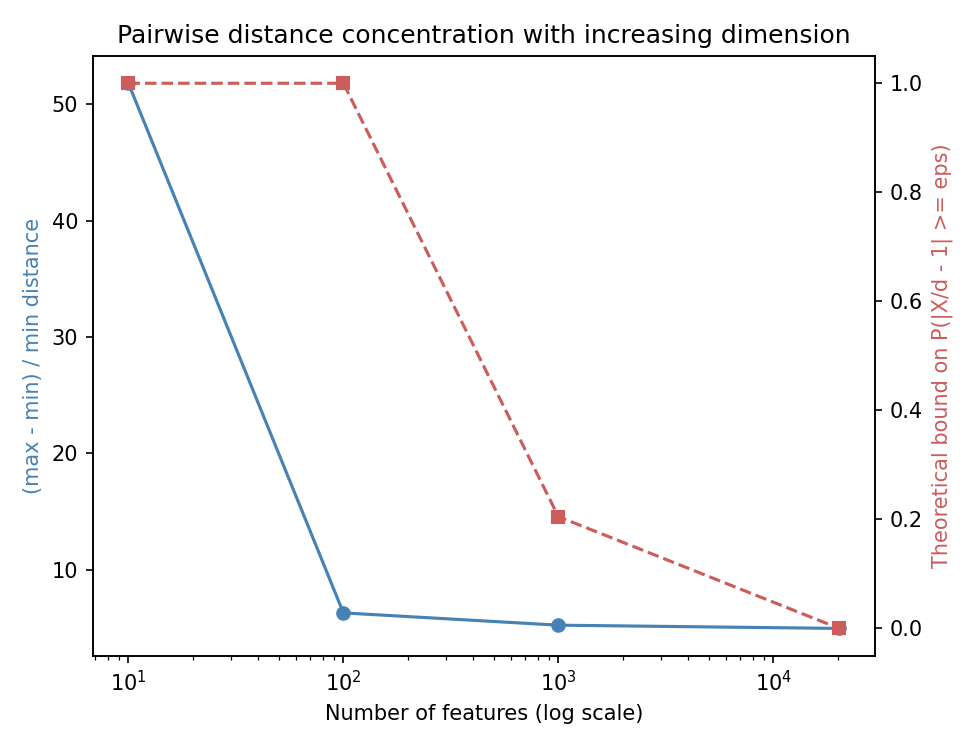
\includegraphics[width=0.62\textwidth]{../figures/distance_concentration.png}
\caption{Relative distance-spread ratio (blue, left axis) and theoretical
tail bound (red, right axis) vs.\ number of features, log-scaled x-axis.}
\label{fig:concentration}
\end{figure}

The concentration ratio drops sharply from $51.79$ at $10$ features to
$6.29$ at $100$ features, then flattens: $5.24$ at $1{,}000$ features and
$4.96$ at all $20{,}264$ genes (Table~\ref{tab:concentration},
Figure~\ref{fig:concentration}). The theoretical bound is vacuous
($\geq 1$) at $d=10$ and $d=100$ -- too few degrees of freedom for the
Chernoff-type bound to be informative -- and only becomes meaningfully tight
at $d=1{,}000$ ($0.205$) and effectively certain at $d=20{,}264$
($1.81\times10^{-20}$). The theory correctly predicts the qualitative
direction (sharp early concentration), but the real data's ratio plateaus
around $\approx 5$ rather than continuing to shrink toward the
near-zero rate the bound implies at $d=20{,}264$ -- direct empirical
evidence that gene co-expression correlation, not the bound's i.i.d.\
assumption, is the dominant factor limiting further concentration once a
few hundred genes are included.

\subsection{Mahalanobis Anomaly Detection}

\begin{figure}[H]
\centering
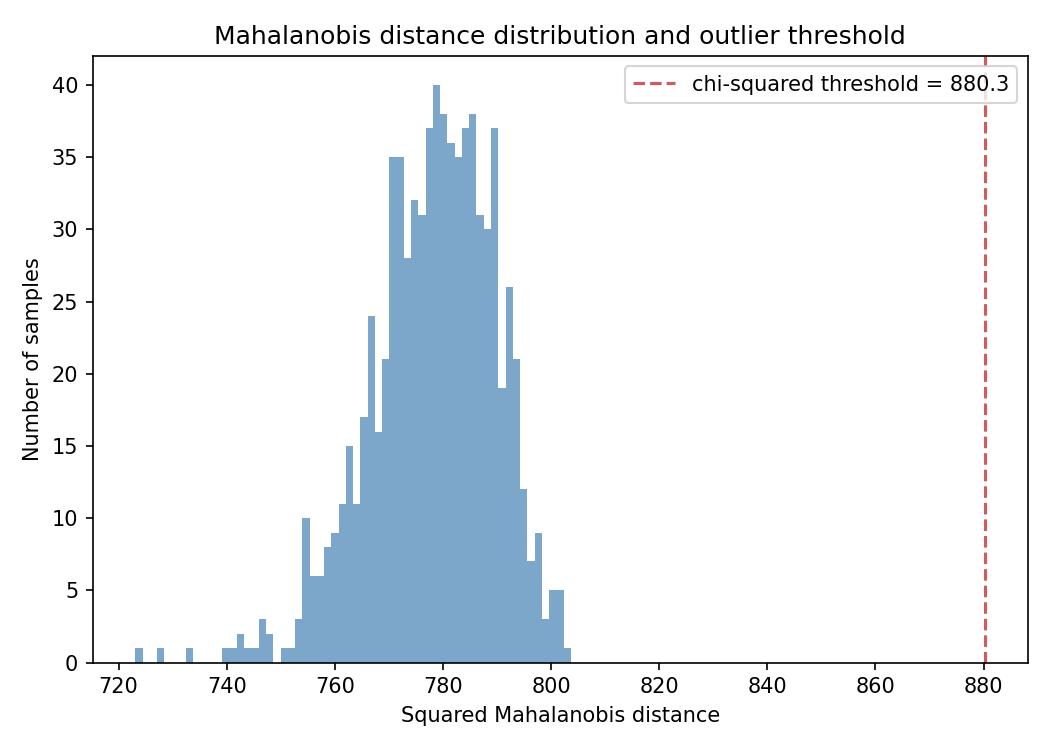
\includegraphics[width=0.65\textwidth]{../figures/mahalanobis_distribution.png}
\caption{Distribution of squared Mahalanobis distances (top-2,000-gene
subset, Ledoit-Wolf shrinkage) across all 801 samples, with the
$\chi^2_{800}$ $97.5\%$-quantile outlier threshold marked.}
\label{fig:mahalanobis}
\end{figure}

\begin{table}[H]
\centering
\caption{Ten samples with the largest squared Mahalanobis distance (none
exceed the formal outlier threshold of 880.28).}
\label{tab:mahalanobis-top10}
\begin{tabular}{lrr}
\toprule
Sample & Cancer type & Squared Mahalanobis distance \\
\midrule
sample\_560 & BRCA & 803.66 \\
sample\_250 & BRCA & 801.93 \\
sample\_599 & LUAD & 801.87 \\
sample\_322 & KIRC & 801.85 \\
sample\_789 & KIRC & 801.69 \\
sample\_497 & BRCA & 801.20 \\
sample\_577 & LUAD & 800.19 \\
sample\_389 & BRCA & 799.99 \\
sample\_77  & KIRC & 799.92 \\
sample\_343 & LUAD & 799.92 \\
\bottomrule
\end{tabular}
\end{table}

The Ledoit-Wolf shrinkage intensity is $\hat\alpha = 0.0239$ -- a light
correction, but sufficient to guarantee invertibility. Squared Mahalanobis
distances range from $723.10$ to $803.66$ (mean $778.10$, std $11.57$),
\emph{all} below the $\chi^2_{800}$ $97.5\%$ threshold of $880.28$ (the
degrees of freedom are the rank of the centered sample covariance,
$n-1=800$, not the feature count $p=2{,}000$, since $D^2$ is confined by
rank to an $800$-dimensional subspace):
\textbf{zero of 801 samples are flagged as outliers.} This is a genuine
empirical finding, not a null result to be explained away: it is discussed
critically in Section~\ref{sec:discussion}. The ten most extreme samples by
raw distance (Table~\ref{tab:mahalanobis-top10}) skew toward BRCA (4 of 10,
vs.\ its $37.45\%$ class share), LUAD (3 of 10, vs.\ $17.6\%$), and KIRC
(3 of 10, vs.\ $18.2\%$), with no PRAD or COAD samples appearing -- with
only 10 samples this is not a statistically robust pattern, but is noted
descriptively.

\section{Discussion}
\label{sec:discussion}

Two results connect directly back to Phase 2's dimension estimates. First,
the fact that t-SNE and UMAP recover near-perfect five-cluster structure
while linear PCA captures only $26.64\%$ of variance in three components
is consistent with Phase 2's own contrast between local, nonlinear-aware
estimators ($D_2 \approx 7.7$, $k$-NN MLE $\approx 29.4$) and the global
linear PCA estimator ($392$ components for $90\%$ variance): the manifold's
true degrees of freedom are low, but they are arranged nonlinearly enough
that no small set of linear directions captures them, exactly the
qualitative signature Phase 2 predicted and this phase now visualizes
directly. Second, the $27$ spectral outliers identified against the
Marchenko-Pastur null (Section~\ref{sec:results}, Table~\ref{tab:spectral-outliers})
give a fourth, independent estimate of ``how many directions carry real
signal'' -- in the same single-digit-to-low-double-digit range as $D_2$
and the $k$-NN MLE mean, and far below the Kaiser-criterion PCA elbow of
$100$, reinforcing that random-matrix theory and local geometric
estimators agree with each other more than either agrees with global
linear variance thresholds.

The zero Mahalanobis outliers deserve a direct methodological explanation
rather than being read as ``the data has no outliers.'' Part of the
explanation is structural rather than biological. Writing
$\ell_1, \dots, \ell_{800}$ for the nonzero eigenvalues of the sample
covariance $S$ and noting $\mu = \mathrm{tr}(S)/p = 1$ because the columns
are standardized, the mean squared Mahalanobis distance satisfies
\begin{equation}
\frac{1}{n} \sum_{i=1}^n D^2(x_i) = \sum_{j=1}^{n-1} \frac{\ell_j}{(1-\alpha)\ell_j + \alpha \mu} \;\leq\; \frac{n-1}{1-\alpha},
\label{eq:mahal-ceiling}
\end{equation}
so with $\hat\alpha = 0.0239$ the mean is bounded above by $819.6$
\emph{no matter what the data are}, and tends to exactly $n-1=800$ as
$\alpha \to 0$. The observed mean of $778.1$ (std $11.57$, a relative
spread of only $1.5\%$) sits exactly where Eq.~\ref{eq:mahal-ceiling} says
it must: this tightness is a property of the $p>n$ geometry, not of these
tumors. Under the corrected $\chi^2_{800}$ threshold of $880.28$ the most
extreme sample (sample\_560, $803.66$) reaches $91.3\%$ of the cutoff, so
the test now has room to fire and still does not. Separately, because the
Ledoit-Wolf target shrinks the covariance toward an isotropic $\mu I$ while
the true correlation-matrix spectrum is extremely heavy-tailed
(Table~\ref{tab:spectral-outliers}: eigenvalues from near-zero to $318.3$),
the blending inflates the estimated variance along the many near-zero
directions more than it deflates it along the few dominant ones, so
$\hat\Sigma_{\text{LW}}^{-1}$ down-weights genuinely informative deviations
relative to an unregularized metric. Mahalanobis distance under heavy
shrinkage is therefore better used here as a \emph{relative ranking} tool
(Table~\ref{tab:mahalanobis-top10}) than as a formally calibrated
significance test -- a limitation of applying an asymptotic threshold to a
deliberately regularized, non-asymptotic $d \gg n$ estimator.

\section{Limitations}
\label{sec:limitations}

The theoretical bounds invoked in this phase all assume some form of
independence or i.i.d.\ structure that real gene-expression data violates
by construction: the Marchenko-Pastur law and the Laurent-Massart
concentration bound (Eq.~\ref{eq:concentration-bound}) are both derived
for i.i.d.\ (or at least uncorrelated) coordinates, whereas genes are
organized into co-expressed pathways with strong pairwise and higher-order
correlations. This is not a flaw in the analysis -- it is precisely the
\emph{point} of comparing real data against these null models: the
$27$ spectral outliers and the plateauing (rather than vanishing)
distance-concentration ratio are both direct, quantified measurements of
how far gene correlation structure pushes the data from the i.i.d.\ null,
not artifacts to be corrected. The Johnson-Lindenstrauss guarantee, by
contrast, makes no distributional assumption about the data itself (only
about the random projection matrix), so its near-exact empirical
satisfaction here is a stronger, assumption-free confirmation. The
Mahalanobis chi-squared threshold assumes asymptotic multivariate
normality of $D^2$ under the estimated covariance, an approximation known
to degrade under heavy shrinkage (Section~\ref{sec:discussion}); a
permutation-based or bootstrap threshold, calibrated empirically rather
than asymptotically, would be a more defensible choice with additional
compute budget. Finally, the $50$-dimensional PCA preprocessing before
t-SNE/UMAP, while standard practice, is itself a design choice that could
mask nonlinear structure concentrated in later linear components; a direct
comparison against unpreprocessed embeddings was not run here for
computational-budget reasons and is left to future work.

\section{References}

\begin{itemize}
\item Johnson, W. B., \& Lindenstrauss, J. (1984). Extensions of Lipschitz
mappings into a Hilbert space. \emph{Contemporary Mathematics}, 26, 189--206.
\item Dasgupta, S., \& Gupta, A. (2003). An elementary proof of a theorem
of Johnson and Lindenstrauss. \emph{Random Structures \& Algorithms},
22(1), 60--65.
\item Marchenko, V. A., \& Pastur, L. A. (1967). Distribution of
eigenvalues for some sets of random matrices. \emph{Mat. Sb.}, 114(4), 507--536.
\item Ledoit, O., \& Wolf, M. (2004). A well-conditioned estimator for
large-dimensional covariance matrices. \emph{Journal of Multivariate
Analysis}, 88(2), 365--411.
\item Laurent, B., \& Massart, P. (2000). Adaptive estimation of a
quadratic functional by model selection. \emph{Annals of Statistics},
28(5), 1302--1338.
\item van der Maaten, L., \& Hinton, G. (2008). Visualizing data using
t-SNE. \emph{Journal of Machine Learning Research}, 9, 2579--2605.
\item McInnes, L., Healy, J., \& Melville, J. (2018). UMAP: Uniform
Manifold Approximation and Projection for dimension reduction.
\emph{arXiv:1802.03426}.
\item Weinstein, J. N., et al. (2013). The Cancer Genome Atlas Pan-Cancer
analysis project. \emph{Nature Genetics}, 45(10), 1113--1120.
\item Dataset: Gene Expression Cancer RNA-Seq (TCGA Pan-Cancer HiSeq),
\url{https://www.kaggle.com/datasets/debatreyadas/gene-expression-cancer-rna-seq}.
\end{itemize}

\appendix
\section{Appendix A: AI Usage Log}
See \texttt{ai\_usage\_log.md} in the repository root for the full,
incrementally maintained log. A Phase 3 entry documenting all
AI-generated modules, representative prompts, and verification steps for
this phase is included there.

\end{document}
